\documentclass{report}

% Packages
%\usepackage[utf8]{inputenc} % Required for German umlauts
\usepackage{amsmath, bm}
% SVG
\usepackage{svg}
% Bib
\usepackage[backend=biber]{biblatex}
\addbibresource{bib/bibliography.bib}
% Geometry
\usepackage{graphicx}
\usepackage{geometry}
\geometry{
  paper=a4paper, % Change to letterpaper for US letter
  inner=2.5cm, % Inner margin
  outer=3.8cm, % Outer margin
  bindingoffset=.5cm, % Binding offset
  top=1.5cm, % Top margin
  bottom=2.5cm, % Bottom margin
}
\setlength{\headheight}{1cm}
\usepackage[onehalfspacing]{setspace}
\usepackage{parskip}
\usepackage{fancyhdr}
\pagestyle{fancy}
\fancyhf{}
\fancyhead[C]{\leftmark}
\fancyfoot[C]{\thepage}
\renewcommand{\headrulewidth}{0.0pt}

%
\usepackage[hidelinks]{hyperref}
%
\usepackage{enumitem} % description alignment
% Chapter title formattting
\usepackage{titlesec}
\titleformat{\chapter}{\huge\bfseries}{\thechapter}{1em}{}

\usepackage{tocbibind}
\settocbibname{References}
%
% Tikz Setup
%
\usepackage{tikz}
\usetikzlibrary{tikzmark}
%\newcommand{\tikzmark}[2]{
%    \tikz[overlay,remember picture,baseline]
%    \node[anchor=base] (#1) {$#2$};
%}
\usetikzlibrary{positioning}
%
% Font
%
\usepackage{fontspec}
\setmainfont{Palatino Linotype}

%
% Custom commands
%
%
% Definition of custom commands
%
\usepackage{xparse}

%%
%% Define commands for formatting C3srMatrix data members correctly
%%
\NewDocumentCommand{\DataMember}{ m o }
  {
  \ifmmode
     \text{#1}\IfNoValueF{#2}{[#2]}
   \else
     #1\IfNoValueF{#2}{[#2]}
   \fi
  }

\NewDocumentCommand{\V}{o}
  {\DataMember{V}[#1]}
\NewDocumentCommand{\VS}{o}
  {\DataMember{VS}[#1]}
\NewDocumentCommand{\J}{o}
  {\DataMember{J}[#1]}
\NewDocumentCommand{\JS}{o}
  {\DataMember{JS}[#1]}
\NewDocumentCommand{\JP}{o}
  {\DataMember{JP}[#1]}
\NewDocumentCommand{\RS}{o}
  {\DataMember{RS}[#1]}
\NewDocumentCommand{\RP}{o}
  {\DataMember{RP}[#1]}
\NewDocumentCommand{\CI}{o}
  {\DataMember{CI}[#1]}


%%%%%%%
%%%%%%% Begin of document
%%%%%%%

\author{\Large{Stanislaw Hüll}\\{Studiengang Master Technische Informatik}\\{Universität Heidelberg - Fakultät für Physik und Astronomie}}
\title{Student Research Project Report}
\date{}
\begin{document}

\begin{minipage}[h]{\textwidth}
\maketitle
\vspace{0.5cm}
\begin{minipage}[h]{\textwidth}
 \centering
 \begin{minipage}{0.3\textwidth}
          \centering
          
\includegraphics[width=0.8\textwidth]{unihd}
        \end{minipage}
        \begin{minipage}{0.4\textwidth}
          \centering
          
\includegraphics[width=0.9\textwidth]{zitihd}
\end{minipage}
\end{minipage}
\vspace{0.5cm}
\begin{abstract}
  Matrix-vector multiplication with sparse banded matrices derived from a structured grid is ubiquitously used for physical simulations in many scientific fields. Implementing the arithmetic using a general purpose sparse matrix format, such as the widely used CSR format, however, yields suboptimal results as the inherent structure of such matrices cannot be exploited by these formats in order to improve the arithmetic performance. This report presents a new sparse matrix storage format, called C3SR format which is based on the CSR format, tailored to maximize the arithmetic performance of matrix-vector multiplication involving sparse banded matrices. Its arithmetic performance is compared against the CSR format using two arithmetic schemes, a CSR-like scheme and a vectorized SIMD scheme on multiple machines displaying large speed-ups due to improved data locality.
\end{abstract}

\end{minipage}

\newpage
\tableofcontents
\newpage
\listoffigures

\chapter{Introduction}

  This section introduces two notions fundamental to the ideas developed in this report, the general purpose \emph{compressed sparse row} matrix storage format (CSR) and, secondly, \emph{sparse banded matrices} as well as their usage in the natural sciences and their particular structure.

  \section{Compressed Sparse Row Matrix Storage Format}

    The compressed sparse row (CSR) format is a widely used storage format for sparse matrices. Unlike other popular sparse matrix storage formats such as the diagonal storage format (DIA), the CSR format is not tailored to any special type of matrix but is a general purpose storage format that makes no assumptions about the matrix's shape or its distribution of non-zeros. The CSR format can be considered an improvement to the naive coordinate format (COO) in that each non-zero's row index is no longer explicitly stored \cite{Bell2011}.

    The CSR format consists of three dense arrays. The values array (V) stores the numerical value for each non-zero entry in the matrix while the associated column index is stored in the column-index array (CI). A third array, the row-pointer array (RP), encodes the beginning of each row's section within the values and column-index arrays, i.e. it stores the offset of each row's first non-zero element into the two arrays. By convention, the row-pointer array usually also contains an additional element denoting the total number of non-zero elements in the matrix. An example for the CSR format is given in Figure \ref{fig:csr_example}.

    \begin{figure}[ht]
      \centering
      \begin{minipage}{0.4\textwidth}
        \centering
        $$
        \begin{pmatrix}
          \color{red}{\bm{3}} &                     0 &  \color{red}{\bm{4}} &                    0 \\
                            0 & \color{green}{\bm{1}} &                    0 &                    0 \\
                            0 &                     0 & \color{blue}{\bm{7}} & \color{blue}{\bm{8}} \\
        \end{pmatrix}
        $$
      \end{minipage}
      \begin{minipage}{0.4\textwidth}
        \centering
        $$
        \begin{matrix}
          \text{Values}  & : & \color{red}{3} &   \color{red}{4} & \color{green}{1} & \color{blue}{7} & \color{blue}{8} \\
          \text{Column-Indices} & : & \color{red}{0} &   \color{red}{2} & \color{green}{1} & \color{blue}{2} & \color{blue}{3} \\
          \text{Row-Pointers} & : & \color{red}{0} & \color{green}{2} &  \color{blue}{3} &               5 &                 \\
        \end{matrix}
        $$
      \end{minipage}
      \caption[Exemplary matrix with corresponding CSR representation.]{\textbf{Exemplary matrix with corresponding CSR representation.} The array elements are color-coded in red for the first row, green for the second row and blue for the third row.}
      \label{fig:csr_example}
    \end{figure}

    Thus, as previously mentioned, the CSR format optimizes the storage requirements of general sparse matrices with respect to the naive coordinate format (COO) shrinking the size of the third array from one entry per non-zero element to a single entry per row irrespective of the row's number of non-zeros. Furthermore, the existing literature, in part, utilizes a different nomenclature referring to the arrays as A (values array), JA (column-index array) and IA (row-pointer array), respectively \cite{sparskit}.

    The CSR format's salient feature is the contiguousness of the rows' non-zero elements' values and column indices making it particularly well suited for matrix-vector-multiplication utilizing a conventional row-by-column computation scheme due to ideal data locality for the values and column arrays. Aside of this characteristic storing the non-zero elements row-by-row as opposed to column-by-column is a choice and thus exist numerical libraries and toolkits such as the Eigen C++ library \cite{eigen:website} or the Harwell-Boeing sparse matrix collection \cite{harwell-boeing} which utilize the CSR format's conjugate, the compressed sparse column format (CSC), as their default means of storing sparse matrices.

    The CSR format serves as a starting point for the C3SR sparse matrix storage format for sparse banded matrices which is the focal point of this work.

  \section{Sparse Banded Matrices Derived from Structured Grids} \label{subsec:structured-grid-matrices}

    Structured grid computations are ubiquitously used for physical simulations in scientific fields such as, for example, computational fluid dynamics, electrodynamics and astrophysics. Generally, a system of partial differential equations is solved by discretization and linearization of the problem which involves generating a grid corresponding to the physical domain in question. A structured grid refers to a mesh whose nodes are uniquely identified by a tuple of coordinates and v.v., such as $(i, j, k)$ for three dimensions (Figure \ref{fig:structured_grid_example}). Such meshes are sometimes referred to as \emph{logically rectangular}.

    \begin{figure}[ht]
        \centering
        \vspace{0.5cm}
        \begin{minipage}{0.4\textwidth}
          \centering
          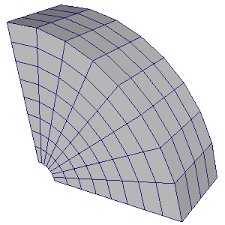
\includegraphics[width=0.9\textwidth]{fig/structured_grid_example.png} % second figure itself
          \caption[Curvi-linear grid over a physically complex domain.]{\textbf{Curvi-linear grid over a physically complex domain.} The grid nodes are logically rectangular despite the non-rectangular physical domain and thus comprise a structured grid. Source: \cite{daad:website}}
          \label{fig:structured_grid_example}
        \end{minipage}\hfill
        \begin{minipage}{0.5\textwidth}
          \centering
          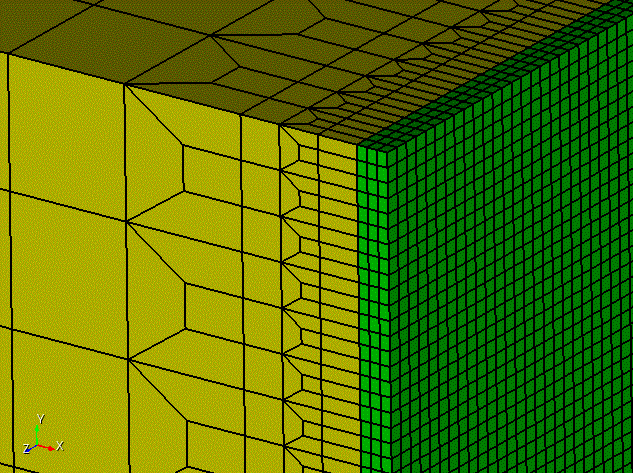
\includegraphics[width=0.9\textwidth]{fig/refined_structured_grid.png} % second figure itself
          \caption[Heterogeneous mesh with structured regions.]{\textbf{Heterogeneous mesh with structured regions.} Outer side (green) and interior volume are fully structured and are connected via an unstructured mesh region. Given proper indexing of grid nodes the resulting sparse matrix will exhibit regularity in the sections pertaining to the structured mesh region. Source: \cite{cubit-mesh-refinement:website}}
          \label{fig:refined_structured_grid}
        \end{minipage}
    \end{figure}

    In contrast to unstructured grids the regularity inherent to structured grids allows for very efficient numerical treatment, such that even in cases where sufficiently complex geometries prohibit the decomposition of the target domain into a single overarching structured grid the domain is often tesselated into an unstructured configuration, with the tiles being filled by independent structured grids \cite{Badcock2000}(Figure \ref{fig:refined_structured_grid}).

    \begin{figure}
        \centering
        \begin{minipage}{0.45\textwidth}
          \centering
          \begin{tikzpicture}[scale=0.75]%[every node/.style={minimum size=1cm},on grid]
\newcommand*{\height}{5}
\newcommand*{\width}{5}
\begin{scope}[every node/.append style={yslant=-0.5},yslant=-0.5]
  \shade[right color=gray!10, left color=black!50] (0,0) rectangle +(\width,\height);

  \foreach \x in {1,...,\width}
    \foreach \y in {1,...,\height}
    {
        \node at (-0.5 + \x, -0.5 + \y) {\pgfmathtruncatemacro\result{21-5*(\x-1)+25*(\y-1)}$\result$};
    }
  \draw (0,0) grid (\height,\width);
\end{scope}
\begin{scope}[every node/.append style={yslant=0.5},yslant=0.5]
  \shade[right color=gray!70,left color=gray!10] (\width,-\height) rectangle +(\height,\width);
    \foreach \x in {1,...,\width}
    \foreach \y in {1,...,\height}
    {
        \node at (\width - 0.5 + \x, -\height + -0.5 + \y) {\pgfmathtruncatemacro\result{1 + 1*(\x-1)+25*(\y-1)}$\result$};
    }

  \draw (\width,-\height) grid (2*\width,0);
\end{scope}
\begin{scope}[every node/.append style={
    yslant=0.5,xslant=-1},yslant=0.5,xslant=-1
  ]
  \shade[bottom color=gray!10, top color=black!80] (2*\width,\height) rectangle +(-\width,-\height);

    \foreach \x in {1,...,\width}
    \foreach \y in {1,...,\height}
    {
        \node at (\width - 0.5 + \x, -0.5 + \y) {\pgfmathtruncatemacro\result{101 + 1*(\x-1)+5*(\y-1)}$\result$};
    }

  \draw (\width,0) grid (2*\width,\height);
\end{scope}
\end{tikzpicture}

        \end{minipage}\hfill
        \begin{minipage}{0.45\textwidth}
            \centering
            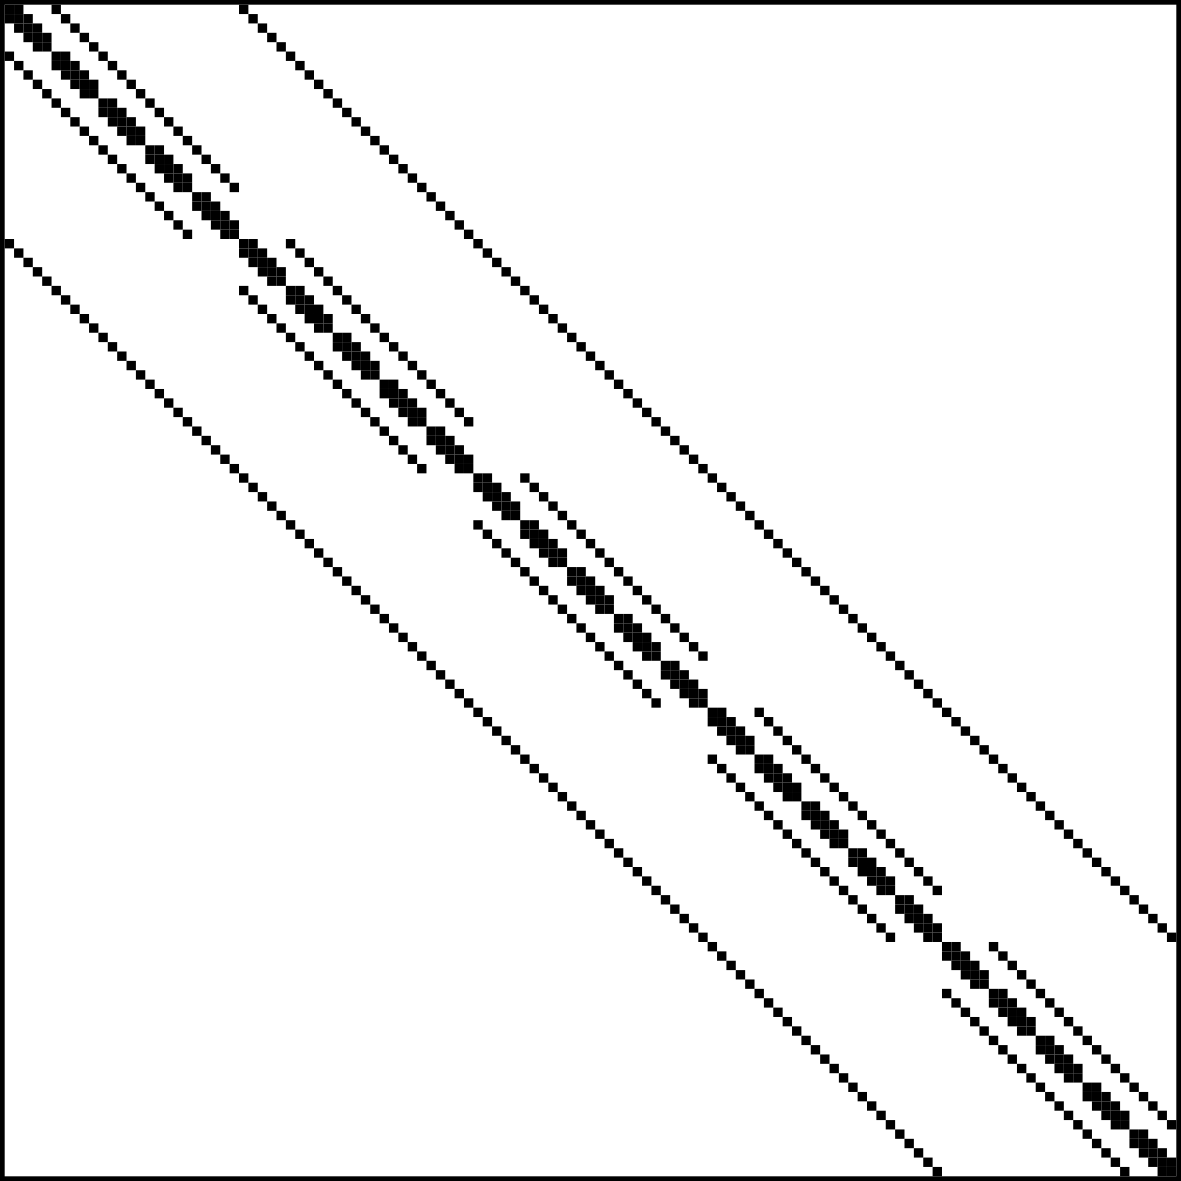
\includegraphics[width=0.9\textwidth]{fig/laplacian_example.png} % second figure itself
        \end{minipage}
        \caption[Structured grid and corresponding matrix for a simple Laplacian.]{\textbf{Structured grid and corresponding matrix for a simple Laplacian} $\nabla^2 u(\vec{r}) = 0$. The Laplace-operator is approximated by the conventional 3-axial symmetric discretization scheme, equivalent to a symmetric 7-point stencil operation.}
        \label{fig:laplacian-example}
    \end{figure}

    The solution procedure yields a sparse linear system whose solution is approximated by iterative methods involving repeated sparse matrix-vector-multiplications $Ax = b$ where the matrix $A$ encodes the adjacency structure of the grid. For a structured grid, the resulting matrix's distribution of non-zeros has a very distinct pattern. Generally speaking, such matrices consist of multiple diagonals of non-zero values at fixed intervals while all other elements are zero. The diagonals are almost fully dense with exceptions arising at positions corresponding to nodes at the grid's boundaries, where the regular adjacency pattern of the grid is disturbed by missing nodes. A grid and its corresponding sparse matrix's structure are depicted in Figure \ref{fig:laplacian-example} for a simple Laplacian problem.

    The matrix's non-zero values depend on the underlying physical problem's parameters, the type of PDE and the differential operators' discretization schemes. In general, the non-zeros' numeric values are independent of their location within the matrix but there exist classes of problems where where the presence of a matrix slice whose rows have diagonal structure implies that those rows share the same numeric values. Furthermore, solving problems on multiple coupled entities such as vectors or matrices yields sparse banded matrices whose 'elements' are themselves square matrices \cite{Godwin2013}.

    The sparse matrices relevant to this work are any sparse matrices that contain one or more sets of rows whose non-zero's column indices are identical save for a fixed offset. Sparse banded matrices arising from the procedure mentioned above have one such set to which the overwhelming majority of rows belong corresponding to all inner grid nodes (such as in the example in Figure \ref{fig:laplacian-example}). However, all of the ideas presented hereinafter may be applied to any sparse matrix whose structure exhibits any degree of repetitiveness.

\chapter{Threefold Compressed Sparse Row Matrix Storage Format}

  Evidently, representing a sparse banded matrix using the regular CSR format is suboptimal, as it has no means of capturing the apparent repetitiveness of the structure. While at first glance the diagonal format might seem an appealing choice for the types of matrices introduced in the previous section, real-life problems produce matrices which are possibly only locally structured, i.e. they contain multiple fully structured sections corresponding to the multiple structured grid regions of the overall heterogeneous domain (Figure \ref{fig:refined_structured_grid}), which need not be aligned in a way to produce a diagonal structure at all. For such matrices the diagonal storage format is suboptimal \cite{Bell2011}. Thus a more flexible approach is taken adapting the general purpose CSR format to better suit the characteristics of sparse banded matrices.

  This section introduces the data layout and the matrix-vector multiplication scheme of the \emph{threefold compressed sparse row} matrix storage format (C3SR). Its raison d'être is to optimize arithmetic performance of matrix-vector multiplications involving sparse banded matrices by improving data locality through a structurally-aware space-saving storage scheme and by implementing an efficient arithmetic scheme capable of profiting from modern computer architectures' hardware assets.

  \section{Data Layout and Storage Scheme}

    It is crucial to observe that, in the most general case, a regularity inherent to a sparse banded matrix's non-zeros' column indices is not shared by the non-zeros' numerical values. While the non-zeros of two or more rows may share the same column indices, save for a possible offset, their corresponding values need not to be similar to each other at all. To prevent that a lack of common regularity impedes optimizing the storage of one or the other it is thus necessary to decouple the representation of a row's non-zeros' column index positions from the representation of their numerical values. The C3SR format accounts for this circumstance and maintains separate data structures for the non-zeros' column indices and their values. Hence the nomenclature of the C3SR format, as it is based on the idea of the CSR format and adds another two potential layers of compression: one for the column indices and one for the values.

    Based on the observation that sparse banded matrices contain many rows whose non-zeros are located at the same positions except for a possible offset the C3SR format decomposes the column-index positions into the column index of the row's first non-zero element, referred to as the \emph{row's peg} hereinafter, and the relative column indices of all of the row's non-zeros with respect to the first non-zero's column index, i.e. the relative offsets with respect to the peg index. The latter column index offsets relative to the peg index shall be called the \emph{row's column index pattern}, or simply the \emph{row's pattern}. Naturally, only unique patterns are stored, drastically shrinking the storage requirements of such matrices whose majority of rows exhibit the same pattern.

    Thus, in order to represent the column indices of a matrix row's non-zeros the C3SR format utilizes three arrays:

    \begin{description}[align = left, labelwidth = 4cm]
      \item [JP - \emph{Peg column indices}] \hfill \\
        Column index of each row's first non-zero. One element per row in matrix.
      \item [J - \emph{Column index patterns}] \hfill \\
        Column index position offsets of the rows' non-zeros relative to the peg column index for each row. Only unique patterns are stored.
      \item [JS - \emph{Patterns' index-pointers}] \hfill \\
        Index-pointer to each row's first element within \J. One element per row in matrix.
    \end{description}

    An example matrix and its corresponding structural information are given in Figure \ref{fig:c3sr_example_structure}.

    \begin{figure}[ht]
      \centering
      \begin{minipage}{0.4\textwidth}
        \centering
        $$
        \begin{pmatrix}
          0 & \bullet & 0 & \bullet & \bullet & 0 \\
          0 & \bullet & 0 & 0 & \bullet & 0 \\
          0 & 0 & \bullet & 0 & \bullet & \bullet \\
        \end{pmatrix}
        $$
      \end{minipage}
      \begin{minipage}{0.4\textwidth}
        \centering
        $$
        \begin{matrix}
          \JP & : & 1 & 1 & 2 &   &   \\
           \J & : & 0 & 2 & 3 & 0 & 3 \\
          \JS & : & 0 & 3 & 0 &   &   \\
        \end{matrix}
        $$
      \end{minipage}
      \caption[Matrix with corresponding C3SR representation (structural information only).]{\textbf{Matrix with corresponding C3SR representation (structural information only).} The non-zeros are denoted as black dots. The $0^{\text{th}}$ and $2^{\text{th}}$ row exhibit the same column index pattern $\big(0,2,3\big)$ at different peg index positions of $1$ and $2$, respectively. Thus the $0^{\text{th}}$ and the $2^{\text{th}}$ element of \JS point \J[0], which is the first element of this unique pattern. The $1^{\text{th}}$ row has a unique pattern which is stored after the previous pattern within \J at offset $3$ which \JS[1] accordingly points.}
      \label{fig:c3sr_example_structure}
    \end{figure}

    The matrix's non-zeros' numerical values are represented using two dense arrays: \V, which contains the actual values and \VS, the index-pointer into \V which relates to \V in the same way \JS relates to \J. The storage in \V is subject to an important property: if multiple rows exhibit the same pattern and their values match at the same time, the values are stored only once within \V. This is a basic requisite for the vectorized matrix-vector multiplication schemes introduced in \ref{subsubsec:vectorized-simd-multiplication-scheme}.

    \begin{description}[align = left, labelwidth = 4cm]
      \item [\V - \emph{Values}] \hfill \\
        Non-zeros' numerical values. Duplicates across rows with the same pattern are stored only once.
      \item [\VS - \emph{Values' index-pointers}] \hfill \\
        Index-pointer to each row's first element within \V. One element per row in matrix.
    \end{description}

    A sixth and final array \RS stores the number of non-zeros in each row of the matrix. This information is required as the index-pointer arrays \JS and \VS point a row's first element within \J and \V but, in contrast to the general CSR format, does not contain the information about how long the segment pertaining to the row within those arrays is. By virtue of the patterns' and values' storage schemes multiple rows' non-zeros' patterns and values may correspond to the very same portion of \J and \V such that the end of that portion cannot be retrieved from the corresponding index-pointer arrays \JS and \VS as could be done for the CSR format by taking the difference of two consecutive index-pointers from \RP.

    \begin{description}[align = left, labelwidth = 4cm]
      \item [\RS - \emph{Row sizes}] \hfill \\
        Number of non-zeros for each row. One element per row in matrix.
    \end{description}

    Another exemplary matrix and its full C3SR format representation are given in Figure \ref{fig:c3sr_example_full}.

    \begin{figure}[ht]
      \centering
      \begin{minipage}{0.4\textwidth}
        \centering
        $$
        \begin{pmatrix}
          1 & 2 & 0 & 3 & 0 & 0 \\
          0 & 1 & 2 & 0 & 3 & 0 \\
          0 & 0 & 4 & 5 & 0 & 0 \\
          0 & 0 & 6 & 7 & 0 & 0 \\
        \end{pmatrix}
        $$
      \end{minipage}
      \begin{minipage}{0.4\textwidth}
        \centering
        $$
        \begin{matrix}
          \JP & : & 0 & 1 & 2 & 2 &   &   &   \\
           \J & : & 0 & 1 & 3 & 0 & 1 &   &   \\
          \JS & : & 0 & 0 & 3 & 3 &   &   &   \\
           \V & : & 1 & 2 & 3 & 4 & 5 & 6 & 7 \\
          \VS & : & 0 & 0 & 3 & 5 &   &   &   \\
          \RS & : & 3 & 3 & 2 & 2 &   &   &   \\
        \end{matrix}
        $$
      \end{minipage}
      \caption[Matrix with corresponding full C3SR representation.]{\textbf{Matrix with corresponding full C3SR representation.} The $0^{\text{th}}$ and $2^{\text{th}}$ rows exhibit the same pattern and the same values, thus the values are stored only once. The last two rows also share a common pattern but with different values.}
      \label{fig:c3sr_example_full}
    \end{figure}

    By design of the storage scheme, sparse banded matrices such as the example shown in Figure \ref{fig:laplacian-example} require very few elements within \J as a structured grid's inner nodes, whose corresponding rows in the sparse banded matrix exhibit the same pattern which is only stored once, comprise the vast majority of all nodes. Depending on the underlying physical problem this property also applies to \V if all rows of an equal pattern share the same set of values. 

    As will be detailed in the following section \ref{subsec:matrix-vector-multiplication-schemes} a matrix-vector multiplication involves copiously accessing \J and \V the C3SR format greatly improves the spatial locality of the data fields most pertinent to arithmetic. A best-case example is given in Figure \ref{fig:c3sr-example-best-case}.

    \begin{figure}[ht]
      \centering
      \begin{minipage}{0.5\textwidth}
        \centering
        $$
        \begin{pmatrix}
          1 & 0 & 2 & 0 & 3 & 4 & 0 & 0 & 0 & 0 \\
          0 & 1 & 0 & 2 & 0 & 3 & 4 & 0 & 0 & 0 \\
            &   & \ddots &   & \ddots &   & \ddots & \ddots \\
          0 & 0 & 0 & 1 & 0 & 2 & 0 & 3 & 4 & 0 \\
          0 & 0 & 0 & 0 & 1 & 0 & 2 & 0 & 3 & 4 \\
        \end{pmatrix}
        $$
      \end{minipage}
      \begin{minipage}{0.4\textwidth}
        \centering
        $$
        \begin{matrix}
          \JP & : & 0 & 1 & 2 & 3 & \cdots & N-1 \\
           \J & : & 0 & 2 & 4 & 5 &        &     \\
          \JS & : & 0 & 0 & 0 & 0 & \cdots &  0  \\
           \V & : & 1 & 2 & 3 & 4 &        &     \\
          \VS & : & 0 & 0 & 0 & 0 & \cdots &  0  \\
          \RS & : & 4 & 4 & 4 & 4 & \cdots &  4  \\
        \end{matrix}
        $$
      \end{minipage}
      \caption[Best-case sparse matrix with corresponding C3SR representation.]{\textbf{Best-case sparse matrix with corresponding C3SR representation.} The matrix exhibits a single pattern and all of its rows have the same values leading to minimally sized \J and \V optimal for the repeated accesses required for matrix-vector multiplication.}
      \label{fig:c3sr-example-best-case}
    \end{figure}

    Note that the structure of a sparse banded matrix derived from a structured grid is exclusively diagonal or locally uniform, i.e. the non-zeros either align into multiple diagonals as in Figure \ref{fig:laplacian-example} or contain blocks of square matrices when solving for multiple coupled entities. Thus the concept of decomposing a row's non-zeros' column indices into its peg index and patterns is slightly redundant but is retained for the sake of flexibility.

  \section{Matrix-Vector Multiplication Schemes} \label{subsec:matrix-vector-multiplication-schemes}

    Aside from the basic CSR-like matrix-vector multiplication scheme, the C3SR format's storage scheme allows for a vectorized arithmetic scheme for sparse banded matrices. This section details the different matrix-vector multiplication schemes whose performance is then gauged in the subsequent section.

    \subsection{Basic CSR-like Multiplication Scheme} \label{subsubsec:basic-csr-like-multiplication-scheme}

      Algorithmically, the basic row-by-column matrix-vector multiplication scheme of the C3SR format is similar to that of the CSR format. Differences arise only in the C3SR's additional offset $\JP[k]$ which is applied to each relative column index prior to accessing the argument vector $x$ as shown in Figure \ref{fig:c3sr_matvecmult_basic}.

      \begin{figure}[ht]
        \centering
        $$
        \begin{matrix}
          \text{CSR}  & : & \sum \limits_{\alpha = 0}^{\RP[k+1] - \RP[k] - 1} & \bigg( & \V[\RP[k] + \alpha]   & \cdot & x\big[\CI[\RP[k] + \alpha]\big] & \bigg)\\
          \vspace{0.3cm} \\
          \text{C3SR} & : & \sum \limits_{\alpha = 0}^{\RS[k] - 1} & \bigg( & \V\big[\VS[k] + \alpha\big] & \cdot & x\bigg[\J\big[\JS[k] + \alpha\big] + \JP[k]\bigg] & \bigg) \\
        \end{matrix}
        $$
        \caption[Matrix-vector multiplication schemes of the C3SR and CSR format in comparison.]{\textbf{Matrix-vector multiplication schemes of the C3SR and CSR format in comparison.} The $k^{\text{th}}$ component of the product $Ax$ is shown. The C3SR format accesses \V and \J from their dedicated index-pointer arrays while the CSR format utilizes one common row-pointer array \RP. Additionally, the C3SR format requires the relative column indices to be offset by the peg column index for each row.}
        \label{fig:c3sr_matvecmult_basic}
      \end{figure}

      As the C3SR format utilizes additional arrays to store index-pointers the number of memory accesses increases likewise. Assuming a general case of a large sparse matrix devoid of any regularity in its structure whose size exceeds the machine's cache capacity the CSR format's arithmetic performance will be better proportional to the difference in the storage size as the above schemes yield memory bound computations involving few trivial arithmetic operations.

      On the flipside, as demonstrated in the previous section sparse banded matrices facilitate very compact storage allowing a small segment of memory, corresponding to possibly only a few cache lines, to contain the matrix's complete structural information and, depending on the underlying physical problem, even the numeric values. This can drastically improve the arithmetic performance of the C3SR format despite the more complex memory access scheme as will be shown in the benchmark section.

    \subsection{Vectorized SIMD Multiplication Scheme} \label{subsubsec:vectorized-simd-multiplication-scheme}

      In addition to the performance gain utilizing the basic CSR-like multiplication scheme due to better data locality, the data layout of a structured matrix in the C3SR format allows for the matrix-vector multiplication to be implemented utilizing SIMD parallelism. The matrix's data is laid out in memory in such a way that the matrix-vector multiplication may be performed for multiple rows at a time using vectorization. Depending on the composition of the matrix corresponding to the types of problems mentioned in the introduction (see \ref{subsec:structured-grid-matrices}) three different but very similar multiplication schemes can be devised.

      \paragraph{SIMD Scheme I: Diagonal structure}

      Suppose that a horizontal slice of rows $r, \ldots, r+k$ has a diagonal structure with the diagonals starting at indices $s, t, \ldots $, such as is depicted in Figure \ref{fig:simd_scheme_diag}. The matrix-vector multiplication for each of the slice's rows is composed of the same number of summands, one per diagonal. Each of the summands is a product of the diagonal's non-zero entry and the argument's corresponding element, starting out with $a_{r,s} \cdot x_s$ for the first diagonal's initial element and $a_{r,t} \cdot x_t$ for the second diagonal. For each subsequent row the matrix element's indices are incremented as well as the argument vector's index, commencing with $a_{r+1, s+1} \cdot x_{s+1}$ for the first diagonal's second element and accordingly for each other diagonal.

      As each diagonal's summand accesses the argument vector's elements in consecutive fashion, for example, $x_s, x_{s+1}, \ldots, x_{s + k}$ for the first diagonal, the access to the argument vector's elements can be vectorized. The other summand's constituents, the diagonal's elements, are stored within \V at a fixed stride which is equal to the number of diagonals. This is due to the fact that the matrix slice's non-zero elements are stored row-by-row while each row has the same number of elements. Thus, for the general case when the rows' values don't match, $a_{r, s}$ is located as many elements before $a_{r+1, s+1}$ within \V as there are diagonals.

      In SIMD terms a stride-gather and a load are required for the diagonal's elements and the argument vector, respectively. The two vector registers are then multiplied and the result is then added onto the next product pertaining to the subsequent diagonal. After the final vectorized addition the result is written into the output buffer using a vectorized store.

      \begin{figure}[ht]
        \centering
        $$
        \begin{pmatrix}
          \\
          \cdots & 0 & a_{r,s} & 0 & \cdots & a_{r,t} & 0 & \cdots & \cdots & \cdots \\
          \cdots & \cdots & 0 & a_{r+1,s+1} & 0 & \cdots & a_{r+1,t+1} & 0 & \cdots & \cdots \\
          \cdots & \cdots & \cdots & 0 & a_{r+2,s+2} & 0 & \cdots & a_{r+2,t+2} & 0 & \cdots \\
          \\
        \end{pmatrix}
        $$
        $$
        \begin{matrix}
          \begin{bmatrix}
            a_{r,s}     \\
            a_{r+1,s+1} \\
               \vdots   \\
            a_{r+k,s+k} \\
          \end{bmatrix} & \cdot & \begin{bmatrix}
                                    x_s      \\
                                    x_{s+1}  \\
                                      \vdots \\
                                    x_{s+k}  \\
                                  \end{bmatrix} & + & \begin{bmatrix}
                                                      a_{r,t}     \\
                                                      a_{r+1,t+1} \\
                                                        \vdots    \\
                                                      a_{r+k,t+k} \\
                                                      \end{bmatrix} & \cdot & \begin{bmatrix}
                                                                                x_t \\
                                                                                x_{t+1} \\
                                                                                \vdots \\
                                                                                x_{t+k}
                                                                              \end{bmatrix} & + & \cdots & = \begin{bmatrix}
                                                                                                                 y_{r} \\
                                                                                                                 y_{r+1} \\
                                                                                                                 \vdots \\
                                                                                                                 y_{r+k}
                                                                                                                \end{bmatrix}\\

        \end{matrix}
        $$
        \caption[Matrix slice with diagonal structure and corresponding vectorized matrix-vector multiplication scheme.]{\textbf{Matrix slice with diagonal structure (above) and corresponding vectorized matrix-vector-multiplication scheme $\bm{Ax = y}$ (below).} A diagonal's elements are located within \V at a fixed stride equal to the number of diagonals. Depending on the hardware capabilities this may make the gather-load operation more performant.}
        \label{fig:simd_scheme_diag}
      \end{figure}

      \paragraph{SIMD Scheme II: Diagonal structure and identical values}

      For the case of a matrix slice whose structure is diagonal and whose rows share the same values, which equates to all values within a diagonal being identical, e.g. $a_{r,s} = a_{r+1, s+1} = \ldots$ for the first diagonal, the previous multiplication scheme is simplified in that the argument vector's values contained in the vector register are simply scaled by the diagonal's value instead of being subjected to a vectorized multiplication (Figure \ref{fig:simd_scheme_diag_collated}). Thus, in contrast to the previous multiplication scheme no SIMD gather is required to compute a matrix-vector product which significantly reduces the operation's comprexity resulting in faster execution times.

      \begin{figure}[ht]
        \centering
        $$
        \begin{pmatrix}
          \\
          \cdots & 0 & a_{r,s} &  0 & \cdots & a_{r,t} & 0 & \cdots & \cdots & \cdots \\
          \cdots & \cdots & 0 & a_{r+1,s+1} & 0 & \cdots & a_{r+1,t+1} & 0 & \cdots & \cdots \\
          \cdots & \cdots & \cdots & 0 & a_{r+2,s+2} & 0 & \cdots & a_{r+2,t+2} & 0 & \cdots \\
          \\
        \end{pmatrix}
        $$
        %$$
        %\V: \begin{pmatrix}
        %  \ldots & a_{r,s} & a_{r,t} & \ldots & \ldots \\
        %\end{pmatrix}
        %$$
        $$
        \begin{matrix}
          a_{r,s} & \cdot & \begin{bmatrix}
                                    x_s      \\
                                    x_{s+1}  \\
                                      \vdots \\
                                    x_{s+k}  \\
          \end{bmatrix} & + & a_{r,t} & \cdot & \begin{bmatrix}
                                                x_t \\
                                                x_{t+1} \\
                                                \vdots \\
                                                x_{t+k}
                                                                              \end{bmatrix} & + & \cdots & =  \begin{bmatrix}
                                                                                                                 y_{r} \\
                                                                                                                 y_{r+1} \\
                                                                                                                 \vdots \\
                                                                                                                 y_{r+k}
                                                                                                                \end{bmatrix}
        \end{matrix}
        $$
        \caption[Matrix slice with diagonal structure and uniform values and corresponding vectorized matrix-vector-multiplication scheme.]{\textbf{Matrix slice with diagonal structure and uniform values (above) and corresponding vectorized matrix-vector-multiplication scheme $\bm{Ax = y}$ (below).} All values within a diagonal are equal simplifying the arithmetic scheme by removing a stride-load operation and a vectorized multiplication in favor of a simple scaling of the argument vector's vector register by the diagonal's value.}
        \label{fig:simd_scheme_diag_collated}
      \end{figure}

      \paragraph{SIMD Scheme III: Uniform structure}

      The third practically relevant case which arises from solving PDEs on multiple coupled entities is matrix slices whose structure is uniform, i.e. each row's non-zero elements are located within the same columns in the matrix slice. This leads to the circumstance that the argument vector's element required for the partial sum involving a matrix column is constant for the whole column (see Figure \ref{fig:simd_scheme_uniform}). Thus the argument vector's elements serve as scaling constants for the vector register containing the matrix's elements, which are again spread at a fixed stride throughout \V. Note that for sparse banded matrices derived from structured grids the values usually differ between rows as the matrix would be singular otherwise. Thus, in practice, the matrix-vector multiplication does not collapse to scalar multiplication.

      \begin{figure}[ht]
        \centering
        $$
        \begin{pmatrix}
          \\
          \cdots & 0 & a_{r,s} &  0 & \cdots & a_{r,t} & 0 & \cdots \\
          \cdots & 0 & a_{r+1,s} & 0 & \cdots & a_{r+1,t} & 0 & \cdots \\
          \cdots & 0 & a_{r+2,s} & 0 & \cdots & a_{r+2,t} & 0 & \cdots \\
          \\
        \end{pmatrix}
        $$
        %$$
        %\V: \begin{pmatrix}
        %  \ldots & a_{r,s} & a_{r,t} & \ldots & a_{r+1,s} & a_{r+1,t} & \ldots & a_{r+2,s} & a_{r+2,t} & \ldots \\
        %\end{pmatrix}
        %$$
        $$
        \begin{matrix}
          \begin{bmatrix}
            a_{r,s}     \\
            a_{r+1,s} \\
               \vdots   \\
            a_{r+k,s} \\
          \end{bmatrix} & \cdot & x_s & + & \begin{bmatrix}
                                              a_{r,t}     \\
                                              a_{r+1,t} \\
                                                \vdots    \\
                                              a_{r+k,t} \\
                                            \end{bmatrix} & \cdot & x_t & + \cdots & = \begin{bmatrix}
                                                                                       y_{r}   \\
                                                                                       y_{r+1} \\
                                                                                       \vdots  \\
                                                                                       y_{r+k} \\
                                                                                     \end{bmatrix}
        \end{matrix}
        $$
        \caption[Matrix slice with uniform structure and corresponding vectorized matrix-vector-multiplication scheme.]{\textbf{Matrix slice with uniform structure (above) and corresponding vectorized matrix-vector-multiplication scheme $\bm{Ax=y}$ (below).} Each non-zero column's elements are located within \V at a fixed stride offset corresponding to the number of non-zero columns. The argument vector's elements serve as scaling constants for the vector register containing the matrix columns' values.}
        \label{fig:simd_scheme_uniform}
      \end{figure}

      All of the arithmetic schemes described above can be extended to vector registers of arbitrary length and are thus theoretically able to scale with additional hardware capabilities. Of course, in order to utilize the above-mentioned computation schemes, a preliminary analysis of the matrix's structure has to be performed in order to determine the segments which can facilitate vectorized arithmetic. Due to the storage scheme of the C3SR format, this can be done very cheaply since if a matrix segment has a diagonal or uniform structure all of the rows exhibit the same pattern and hence the same values in \JS. For uniformly structured segments all peg indices are identical, while for a diagonally structured segment the peg indices are consecutive integers. Additionally, if the rows' values are identical for the case of a diagonal structure the rows' index-pointers \VS are also identical.

\chapter{Performance Benchmarks}

  The matrix-vector multiplication performance of the C3SR format is measured in its CSR-like and vectorized implementations (see \ref{subsec:matrix-vector-multiplication-schemes}). Firstly, baseline performance is established by comparing the matrix-vector multiplication performance of the C3SR format's CSR-like multiplication scheme introduced in \ref{subsubsec:basic-csr-like-multiplication-scheme} against the CSR format's performance on different sparse banded matrices derived from structured grids and on three different machines. Secondly, the C3SR format's baseline performance is compared against its vectorized counterpart introduced in \ref{subsubsec:vectorized-simd-multiplication-scheme}.

  The following subsection introduces the sparse banded matrices used for the performance benchmarks and their method of acquisition. Subsequently, the results of the performance benchmarks are discussed. Information on the machines used for the benchmarks can be found at the ASC infrastructure wiki\footnote{https://mp-force.ziti.uni-heidelberg.de/kmbeutel/personal-wiki/wikis/ASC-infrastructure} (the KNL was configured to 50\% hybrid mode). All benchmarks were run multi-threaded utilizing the machines' full hardware capabilities.

  \section{Generation of Sparse Banded Matrices as Test Matrices}

    For the purpose of gauging the arithmetic performance, test matrices are created. These matrices resemble the structure of the sparse banded matrices introduced above and are created by iterating through a 3D grid of fixed integral dimensions X, Y, Z and applying a given stencil operation which encodes the desired adjacency relationship of the grid. Nodes requested by the stencil but missing from the grid, i.e. nodes on the grid's outer borders, are omitted, i.e. their corresponding entries in the adjacency matrix carry a zero corresponding to Dirichlet-type boundary conditions.

    The matrix's non-zero entries' numeric values are obtained from evaluating a sinusoidal function at the geometric center point $\vec{r} = (x, y, z)$ inbetween the two nodes in question whereby each Cartesian component $x, y, z$ is scaled by its coordinate's span $X, Y, Z$. An additional offset serves to prevent that entries in the matrix correponding to adjacent nodes according to the stencil incidentally evaluate to 0. The function utilized is $$W(x,y,z; n_x, n_y, n_z) = 2 + \sum \limits_{d \in \{x,y,z\}} \sin{\frac{d}{d_{\text{max}}} \cdot \pi \cdot n_d} $$ where $n_x, n_y, n_z$ are periodicity parameters for each dimensions. The matrix in Figure \ref{fig:laplacian-example} has been created using this method.

    Note that $n_d = 0 \Leftrightarrow \partial_d W(\vec{r}) \equiv 0$, introducing a periodicity in the corresponding dimension $d$. This feature is utilized to control the periodicity in the matrix's values.

    For the purpose of this work two different sets of parameters are utilized generating two different matrices: A smaller matrix generated from a $100 \times 100 \times 100$ grid with the periodicities $n_x = n_y = n_z = 0$ and a second matrix based on the same grid but different periodicities $n_x = 1.1; n_y = 1.2; n_z = 1.3$. Both matrices are generated from a symmetric 7p-stencil operation. The matrices' structures are their grid's equivalent to the example shown in Figure \ref{fig:laplacian-example}.

    The first matrix's values are identical for all rows whose pattern is the same such that \V and \J contain the same small number of elements. The second matrix's rows' values are all unique and thus \V contains approximately $7 \cdot 100^3$ elements (Figure \ref{fig:matrix_stats}).

    \begin{figure}[ht]
      \centering
      \begin{tabular}{ l | c c }
          Array & First Matrix & Second Matrix       \\
        \hline                                       \\
        \V         & $135$          & $6940000$      \\
        \VS        & $1000000$      & $1000000$      \\
        \J         & $135$          & $135$          \\
        \JS        & $1000000$      & $1000000$      \\
        \JP        & $1000000$      & $1000000$      \\
        \RS        & $1000000$      & $1000000$      \\
        Total Size in C3SR format & $\approx 16$MB & $\approx 72$MB \\
        Total Size in CSR Format & $\approx 87$MB & $\approx 87$MB \\
        \hfill
      \end{tabular}
      \caption[Matrices in C3SR format used for matrix-vector multiplication benchmarking.]{\textbf{Matrices in C3SR format used for matrix-vector multiplication benchmarking.} Number of elements is displayed for each array. \V stores double-precision floating-points while all other arrays use 32 bit-wide integers. Additionally, the matrix's size in CSR representation is listed.}
      \label{fig:matrix_stats}
    \end{figure}

    Note that the two matrices share the same structure and thus their only difference is found in \V and \VS. Concerning the vectorized matrix-vector multiplication scheme the first matrix primarily utilizes scheme II (Figure \ref{fig:simd_scheme_diag_collated}) while the second matrix mainly relies on scheme I (Figure \ref{fig:simd_scheme_diag}). The matrices are generated using the asc::matrixgen C++ library\footnote{https://mp-force.ziti.uni-heidelberg.de/asc/AscMatrixGen}.

  \section{Performance of CSR-like Matrix-Vector Multiplication}

    The C3SR format's CSR-like matrix-vector multiplication scheme (referred to as \emph{baseline implementation} hereinafter; see \ref{subsubsec:basic-csr-like-multiplication-scheme}) is compared against its CSR format's pendant using the Eigen C++ library \cite{eigen:website} on three different machines using the sparse banded matrices introduced in the previous section. The results are displayed in Figure \ref{fig:baseline_arithmetic_performance}.

    \begin{figure}[!ht]
      \centering
      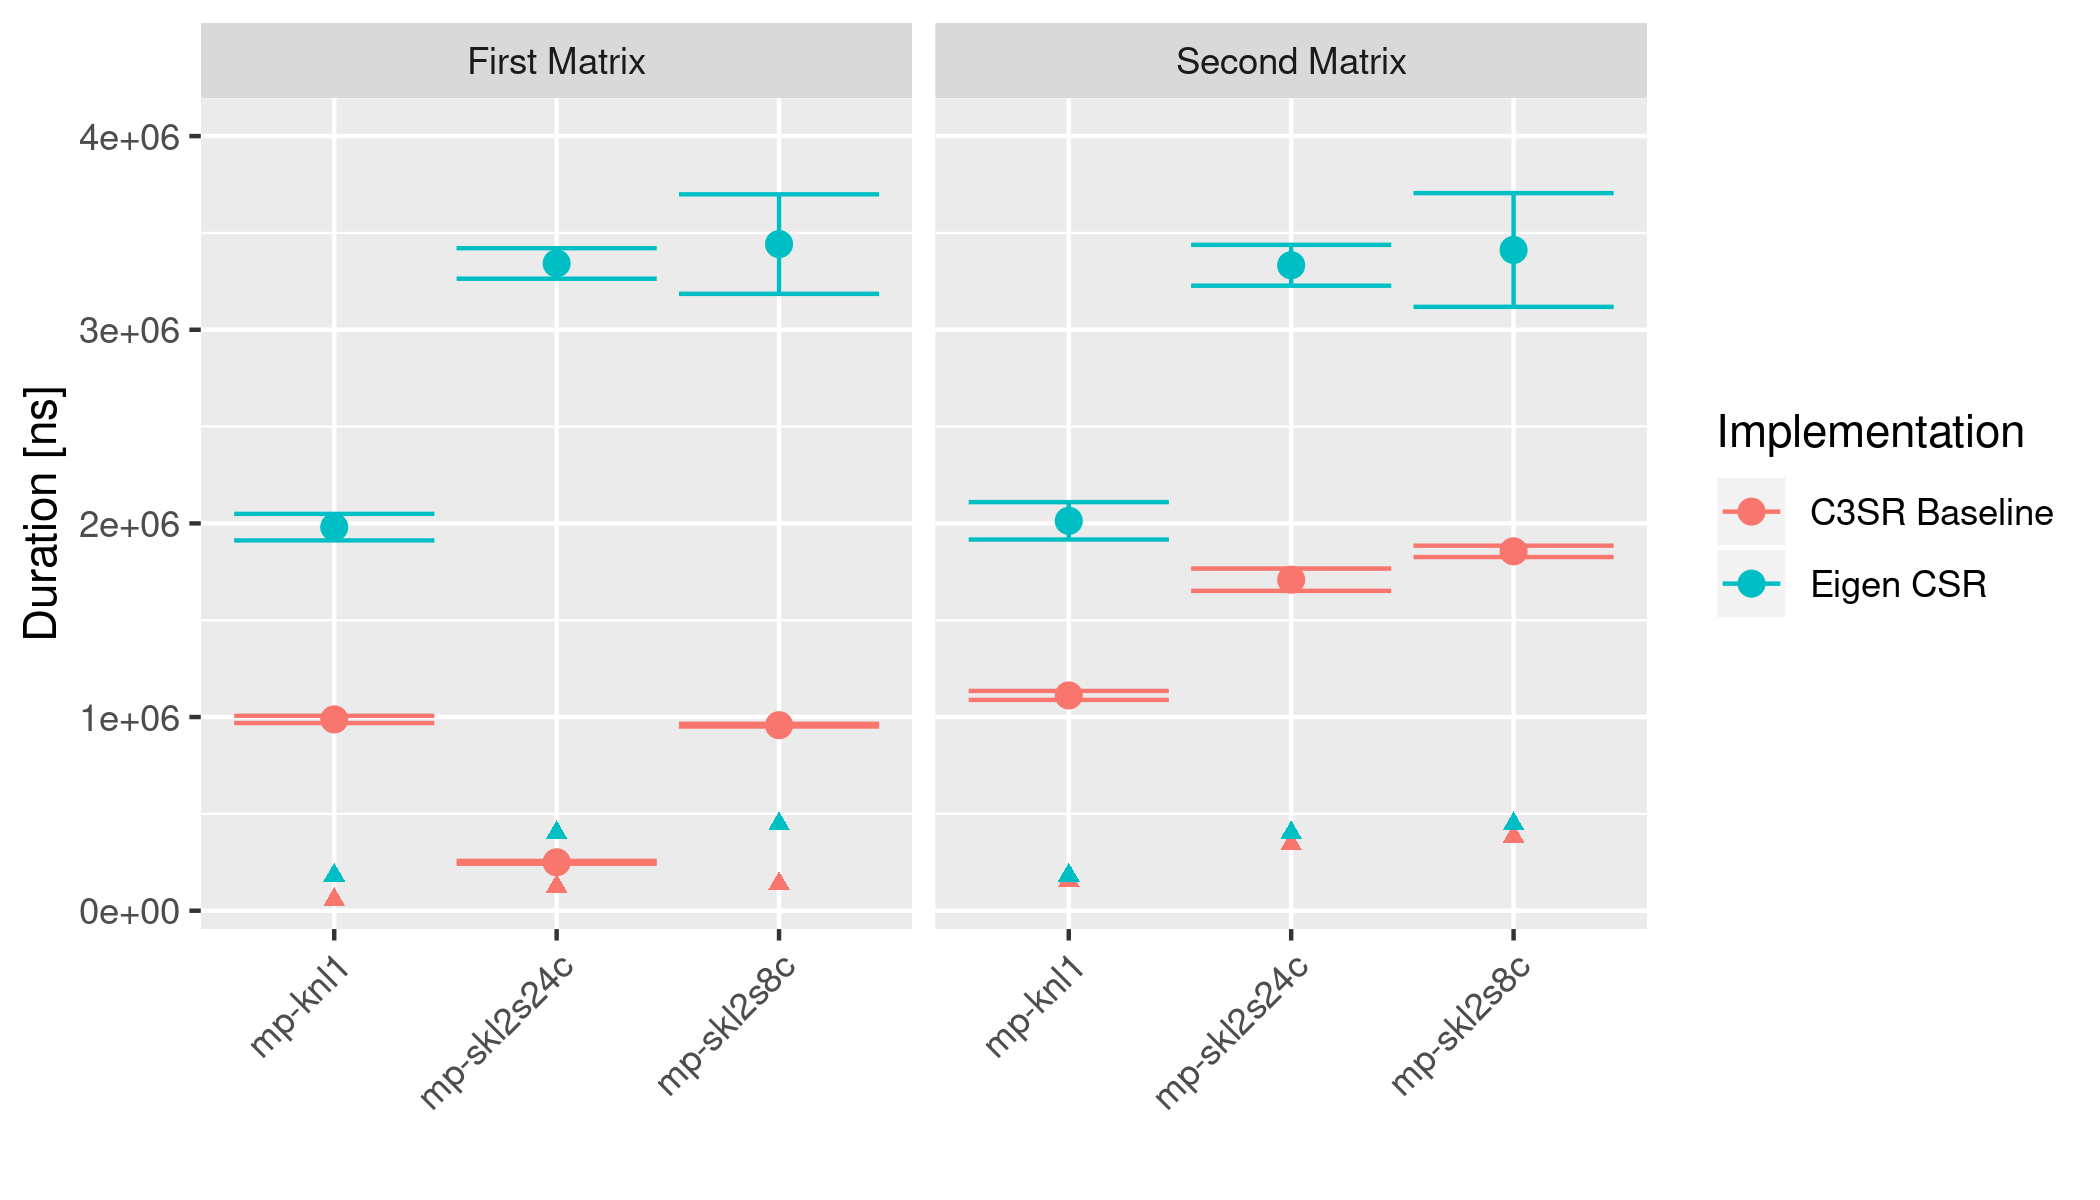
\includegraphics[width=0.9\textwidth]{assets/eigen_vs_c3sr_baseline}
      \caption[Performance comparison of the CSR format against the C3SR format on sparse banded matrices.]{\textbf{Performance comparison of the CSR format against the C3SR format on sparse banded matrices.} The means and sample standard deviations of $10$ samples à $10000$ consecutive matrix-vector multiplications are shown. As the CSR format's representation of the different matrices is identical except for differing numeric values the arithmetic performance is the same save for statistical variance. The triangular symbols denote the theoretical limits as determined by the quotient of the total amount of data involved in a matrix-vector multiplication and the system's theoretical memory bandwidth.}
      \label{fig:baseline_arithmetic_performance}
    \end{figure}

    By design of the C3SR format, it outperforms the CSR format in the order of magnitude of around $50\%$ irrespective of the machine. This is due to the reduction in the size of the representation of the matrices and the consequent improvement in data locality as the C3SR format's arithmetic is slightly more complex as discussed in \ref{subsubsec:basic-csr-like-multiplication-scheme}. Accordingly, the performance improvement is more pronounced for the first matrix, whose storage size is smaller, entailing speed-up factors of approximately 2, 13, and 3.

    Despite the clear performance benefits the above results have to be qualified further as the implementation of the C3SR format\footnote{https://mp-force.ziti.uni-heidelberg.de/shuell/c3srmatrix} uses a NUMA-aware memory allocation scheme for its data arrays, correctly distributing them across physical memory, suitable for the multi-socket systems utilized for the benchmarks. Conversely, the Eigen C++ library, a general purpose linear algebra and numerics framework, does not tailor its data fields' memory layout in such a way that might lead to performance penalties due to a data distribution inadequate for the access patterns of the multi-threaded arithmetic. Additionally, Eigen internally uses the multi-threading framework OpenMP \cite{openmp:website} which entails a dynamic overhead not present in the implementation of the C3SR format.

  \section{Performance of SIMD Matrix-Vector Multiplication}

    The C3SR format's vectorized multiplication scheme's performance is measured by comparing it against the baseline performance. The implementation of the vectorized multiplication scheme utilizes the explicit SIMD vectorization library UME::SIMD \cite{umesimd2017}. The results are displayed in Figure \ref{fig:arithmetic-performance}.

    \begin{figure}[!ht]
      \centering
      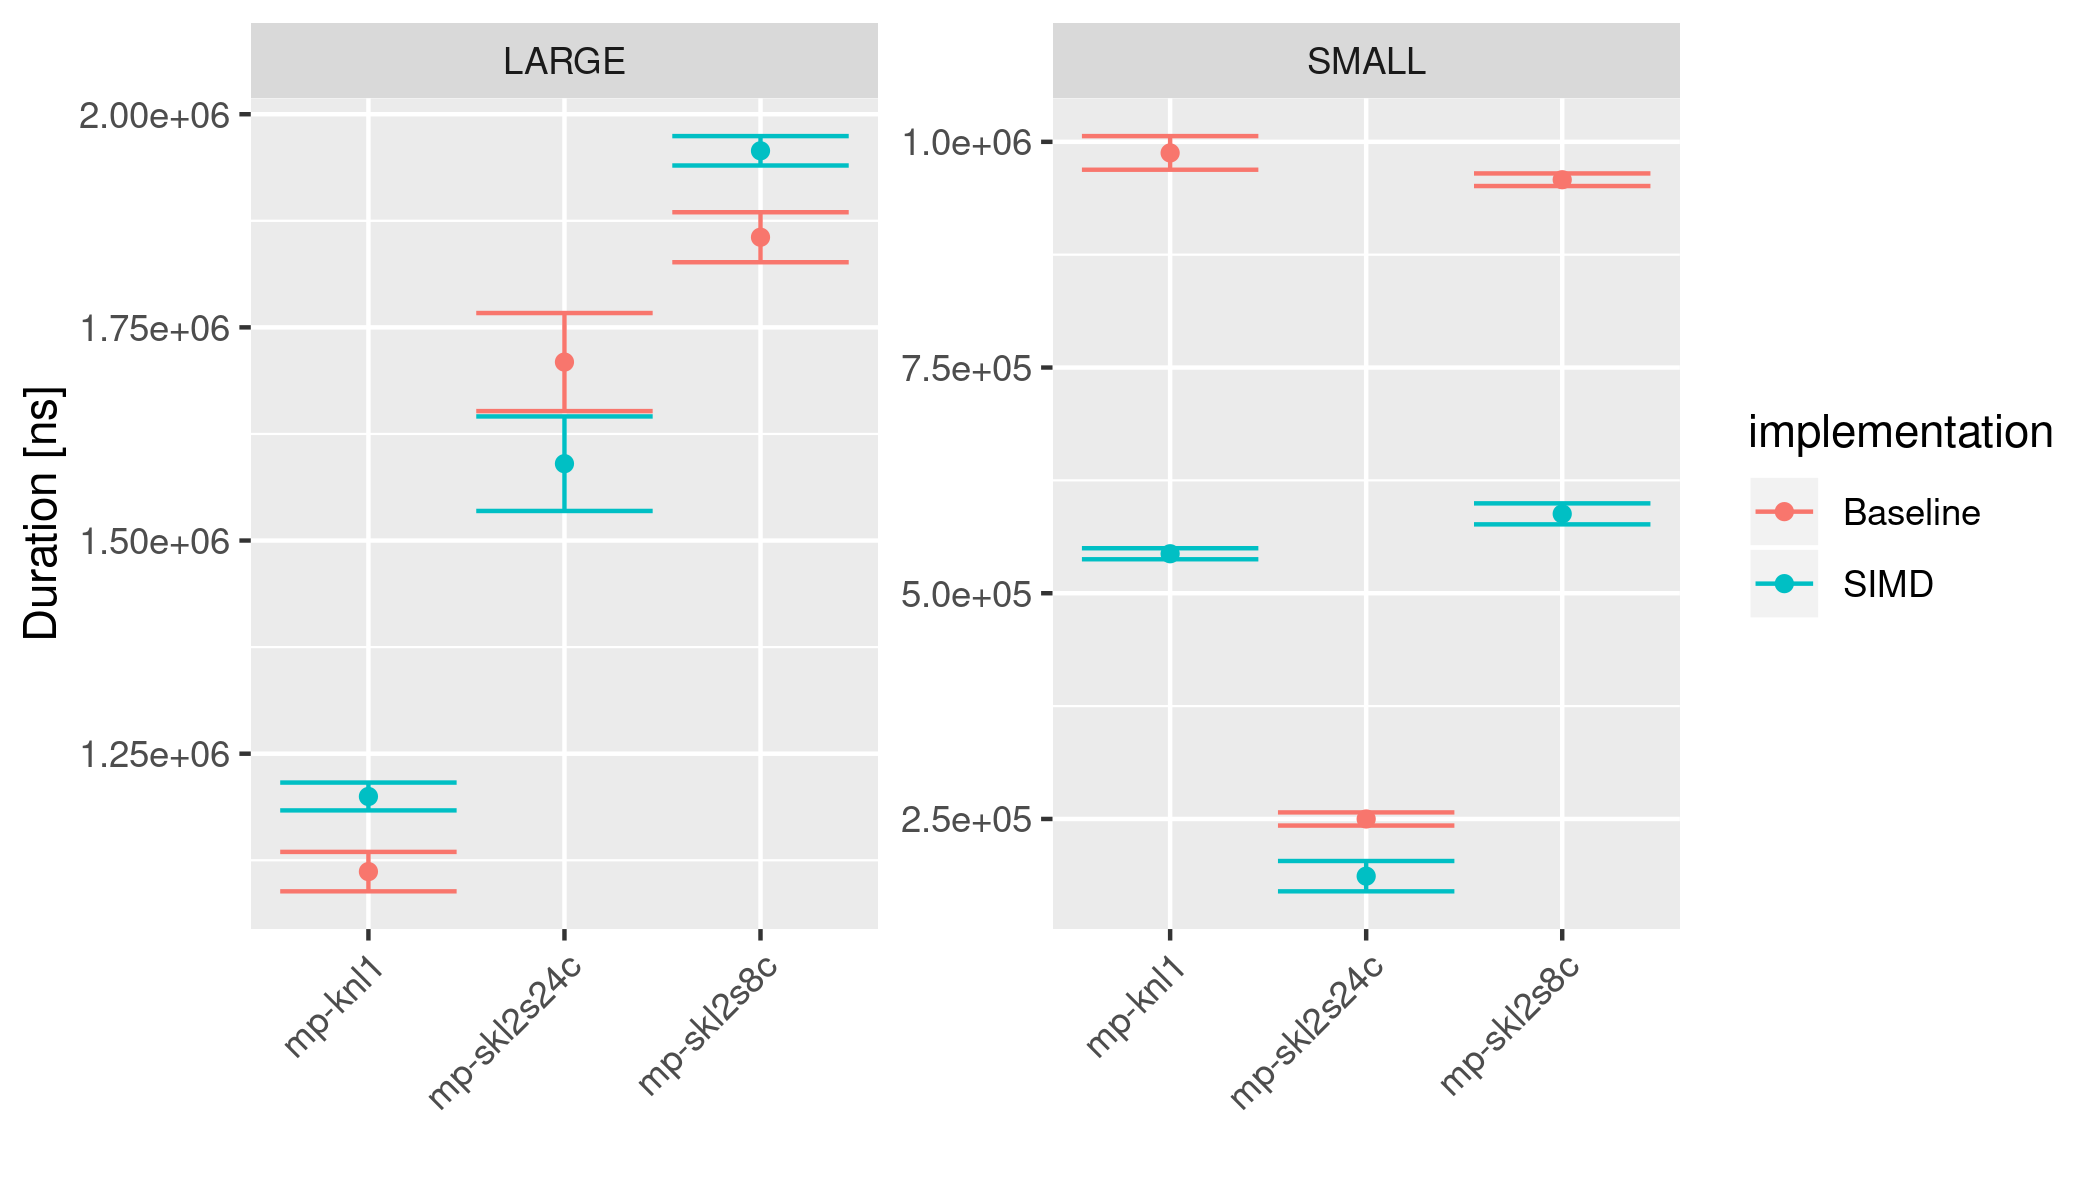
\includegraphics[width=0.9\textwidth]{assets/arithmetic_performance}
      \caption[Performance of C3SR vectorized matrix-vector multiplication scheme compared to baseline implementation.]{\textbf{Performance of C3SR vectorized matrix-vector multiplication scheme compared to baseline implementation.} The means and sample standard deviations of $10$ samples à $10000$ consecutive matrix-vector multiplications are shown.}
      \label{fig:arithmetic-performance}
    \end{figure}

    Sparse matrix-vector multiplication is a memory-bound computation so that the efficacy of a vectorized arithmetic implementation depends very strongly on the amount of data that is required to be read from memory and whether the dynamic overhead involved in determining the applicable SIMD scheme is compensated by a speed-up in arithmetic. This fact is reflected in the measurements as for the second matrix the SIMD implementation is generally slower than the baseline implementation. Only for the first matrix a significant speed-up can be observed on every machine. However, this might be partly due to the fact that the second matrix's SIMD multiplication scheme is less performant as it involves strided loads from memory which might equate to regular gather operations on the hardware used for this benchmark (see \ref{subsubsec:vectorized-simd-multiplication-scheme}).

  \section{Further Considerations}

    By evidence of the performance benchmarks presented in the previous section the basis for the performance gain in the arithmetic of the C3SR format with respect to the CSR format for sparse banded matrices is the reduction of the matrix's total storage size in memory leading to big improvements in data locality during matrix-vector multiplication.

    The C3SR format's storage scheme is tailored to minimize the matrix' storage size in memory. However, depending on how the matrix object is created in memory, adhering to the storage scheme to its full extent may not be optimal as it might limit parallelism during object construction. The data arrays' contents are strongly coupled such that the workload cannot be trivially spread across multiple threads. Instead, it might be advisable to partition the matrix into equally sized slices whose independent C3SR objects can be created in parallel. Finally, these distinct C3SR objects corresponding to the matrix slices are then transformed into a singular object by concatenating the data arrays requiring that the index-pointer arrays are offset by the number of rows preceding their first matrix row.

    In order to establish an estimate for an apt partition size Figure \ref{fig:structured_grid_matrix_heap_size} displays the total storage size depending on the partition size for the two matrices used for the performance benchmarks. It is evident that there exists a point of diminishing returns past whose partition size there is no significant gain in storage size reduction. This point is reached when the sizes of \V and \J, the two arrays responsible for the reduction in storage size for the C3SR format, fall significantly below the fixed sizes of the remaining arrays, which constitute a minimum to the storage size.

    Thus, the performance benefits of the C3SR format may be kept even when trading larger storage sizes in favor of the parallelizability of the application.

    \begin{figure}[ht]
      \centering
      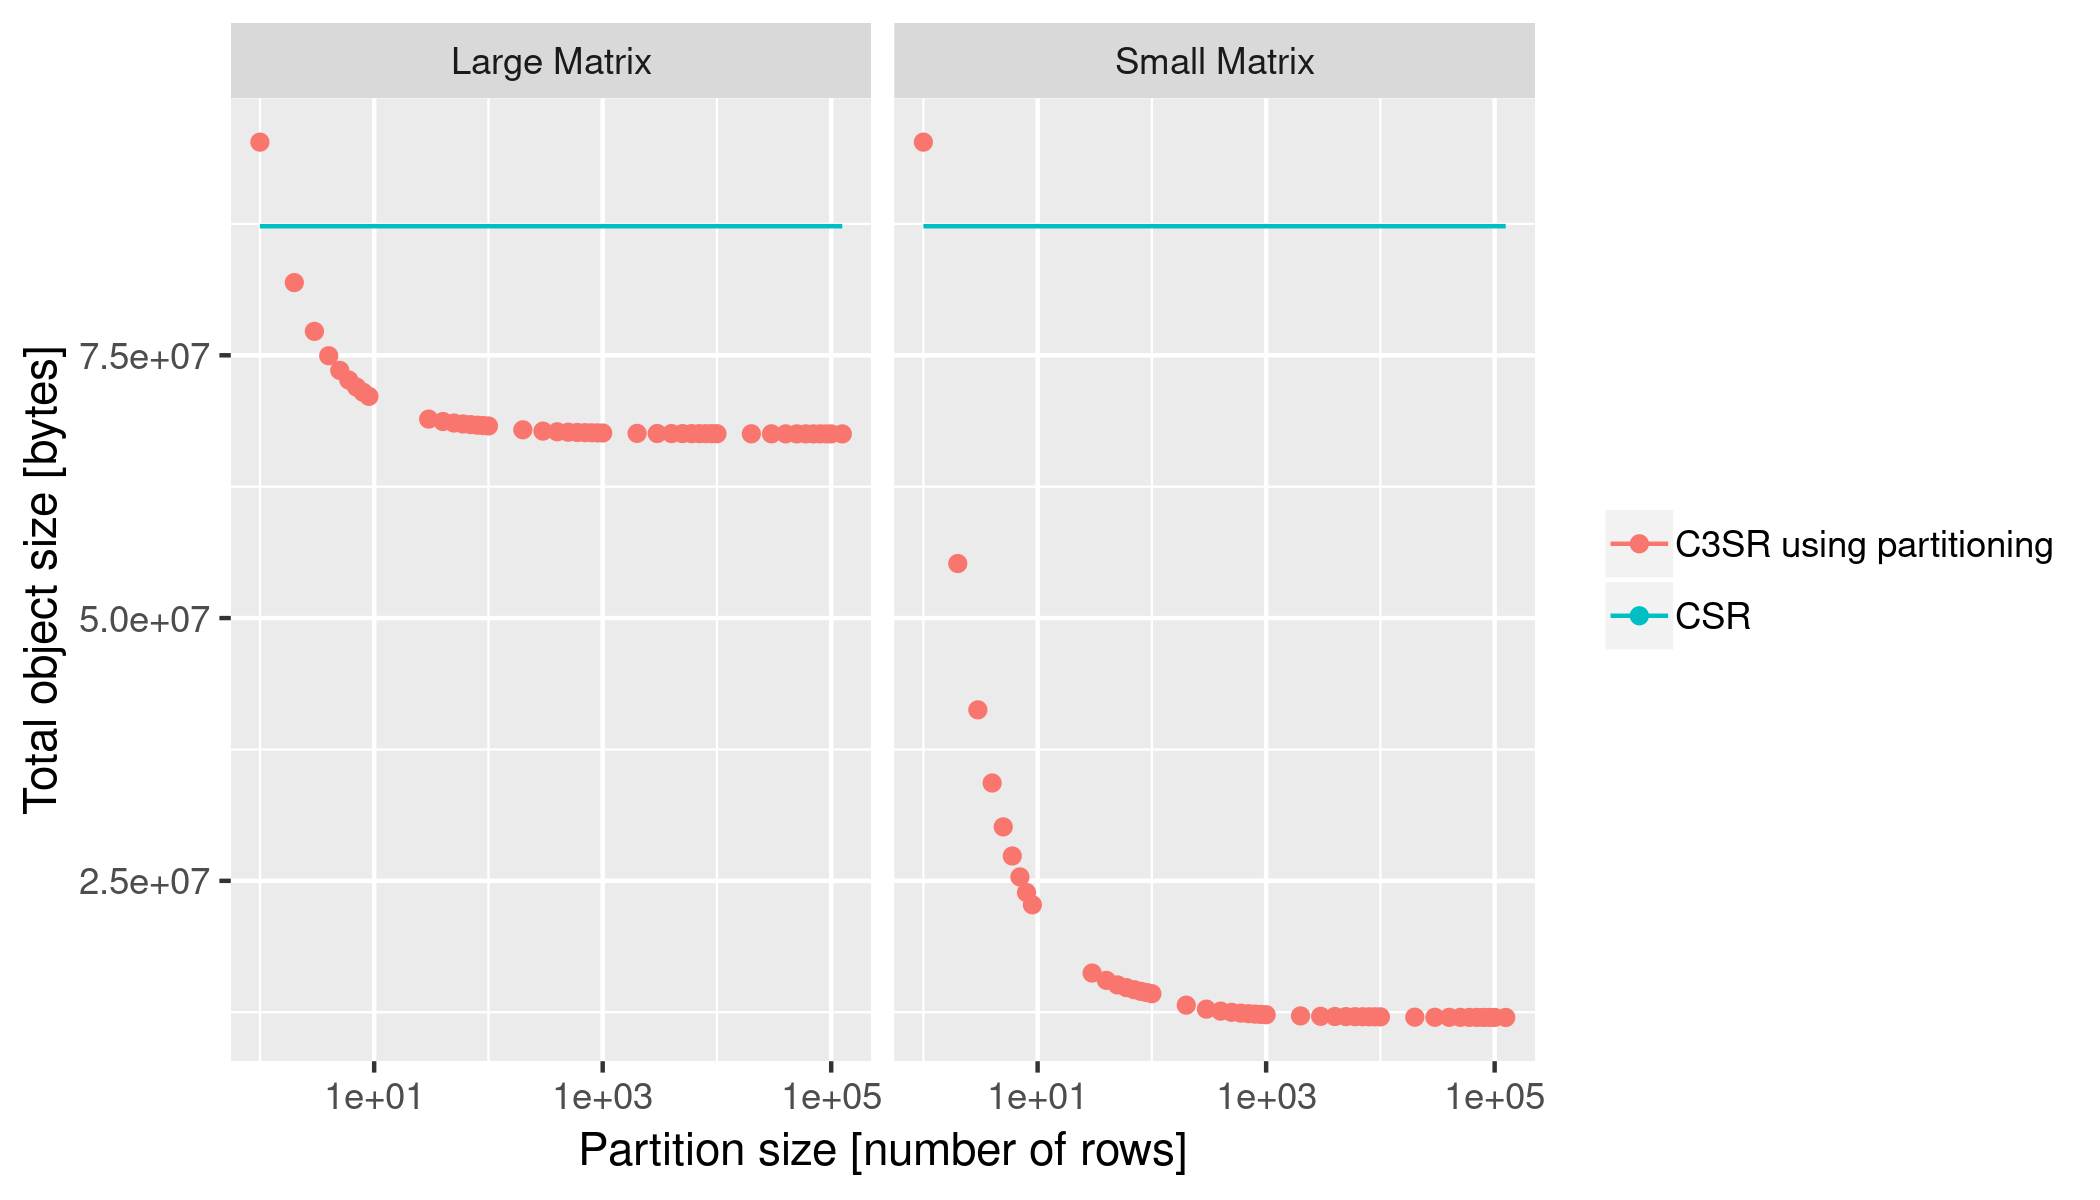
\includegraphics[width=0.9\textwidth]{assets/structured_grid_matrix_heap_size}
      \caption[C3SR matrix storage size depending on partition size]{\textbf{C3SR matrix storage size depending on partition size.} Numeric values are stored using double precision floating-point numbers while all other arrays utilize 32 bit integers. A point of diminishing returns is reached at a partition size of around 1000, past which the storage size in memory does not shrink significantly. Thus, creating C3SR objects using partition sizes of 1000 and larger may yield a similar performance while speeding up the creation of the object. For comparison the corresponding CSR format's storage size is provided.}
      \label{fig:structured_grid_matrix_heap_size}
    \end{figure}

\begingroup
\let\clearpage\relax
\chapter*{Conclusion}
\endgroup
\markboth{Conclusion}{Conclusion}
\addcontentsline{toc}{chapter}{Conclusion}

  This report introduces the threefold compressed sparse row matrix storage format (C3SR) which has been designed to adapt the CSR format to improve the performance of matrix-vector multiplication for sparse banded matrices derived from structured grids. Significant performance benefits have been demonstrated for two different sparse banded matrices based on a $100 \times 100 \times 100$ grid utilizing the basic CSR-like matrix-vector multiplication scheme of the C3SR format.

  A vectorized arithmetic scheme could only be shown to provide performance improvements for the matrix whose storage size in memory is significantly smaller implying that the matrix-vector multiplication is bound by the system's memory bandwidth. Thus, for the machines utilized for this work, the applicability of vectorization for the arithmetic depends strongly on the sparse banded matrix in question. For some systems, it showed worse performance than the baseline CSR-like implementation.

  \section*{Future Work}

    In order to gauge arithmetic performance, this project uses few synthetic matrices which, albeit being realistic examples, cover only very little of the total spectrum of sparse banded matrices that occur in real-life applications. Especially heterogeneous domains as discussed in section \ref{subsec:structured-grid-matrices} yield sparse matrices which are only partially structured. These scenarios have to be investigated separately in terms of arithmetic performance.

\printbibliography
\addcontentsline{toc}{chapter}{\bibname}

\end{document}
